\documentclass[a4paper,12pt]{article}

\usepackage{cmap}
\usepackage[T2A]{fontenc}
\usepackage[utf8]{inputenc}
\usepackage[english,russian]{babel}


\usepackage{graphicx}
\graphicspath{ {./images/} }

\author{lauraep}
\title{Calc v1.0}

\begin{document}
	\maketitle

	\section{Онсовные функции}
		Арифметические операторы
		
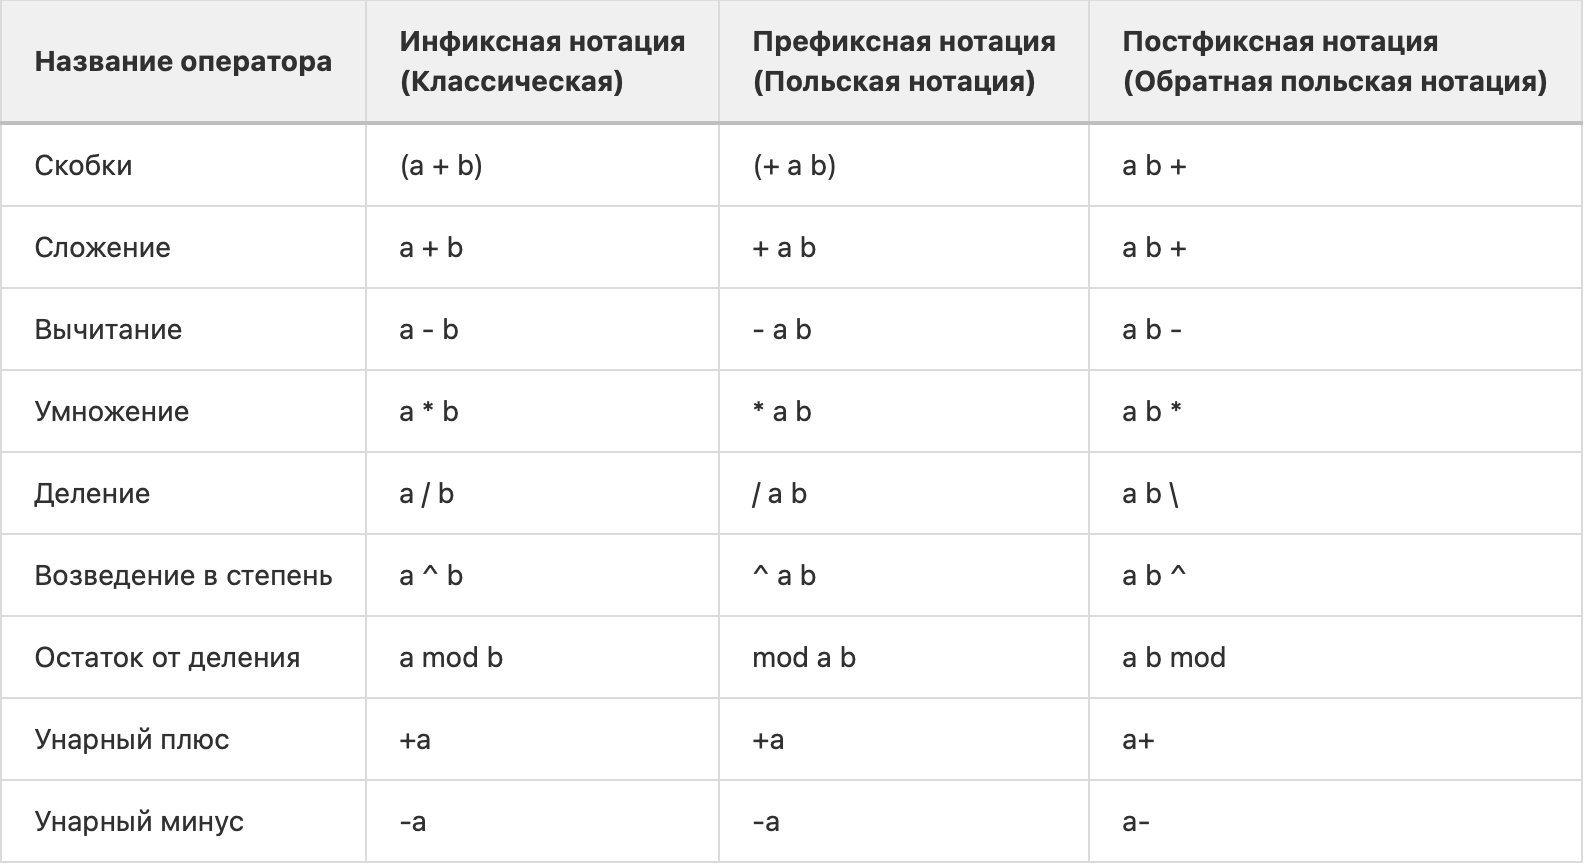
\includegraphics[scale = 0.3]{phunc}
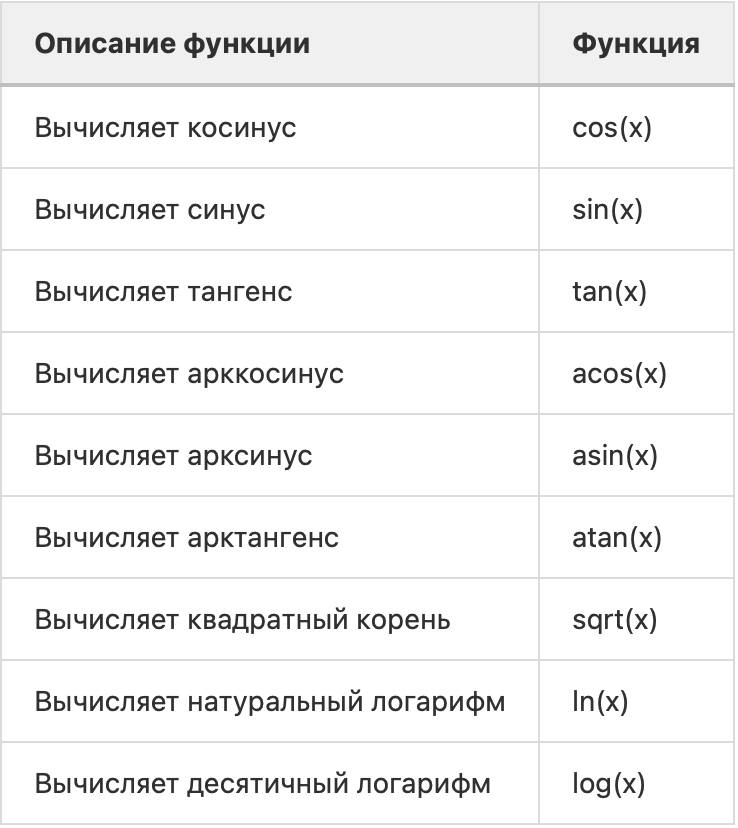
\includegraphics[scale = 0.3]{trig}
	
	\begin{itemize}
		
\itemОбласть определения и область значения функций ограничиваются по крайней мере числами от -1000000 до 1000000
	
\itemПроверяемая точность дробной части - минимум 7 знаков после запятой
	У пользователя должна быть возможность ввода до 255 символов
\end{itemize}
	
	\section{Работа с калькулятором}
	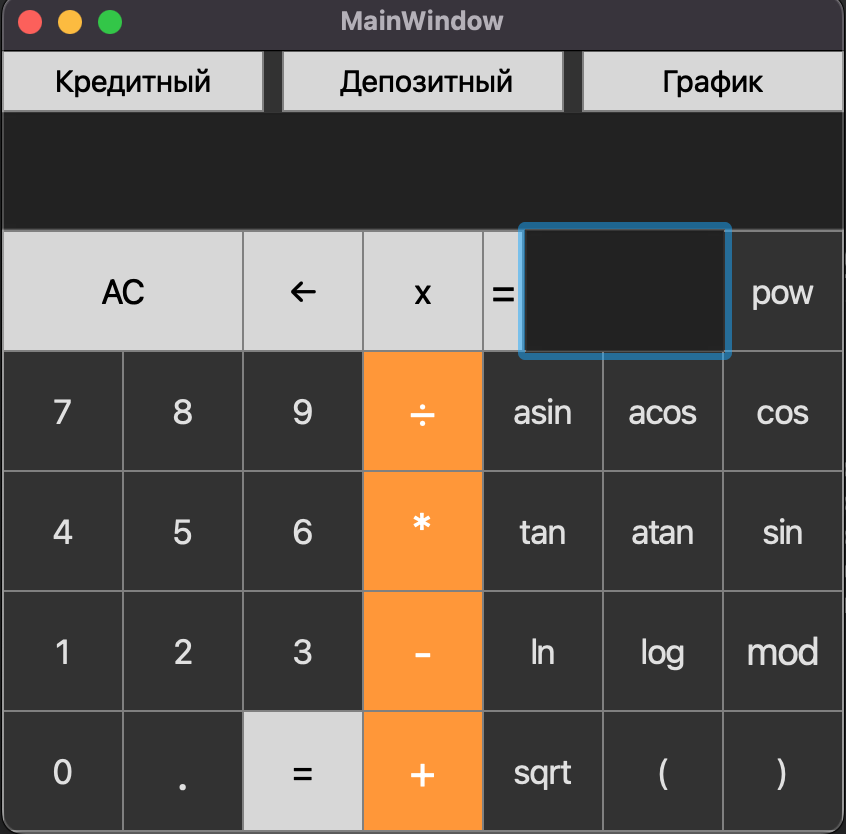
\includegraphics[scale = 0.7]{calc}
	
		\begin{itemize}
		
		\item Можно вводить переменную  X    в поле ввода её значение

		
		\item Примеры вводятся как ручками с лавиатуры, так и с помощью кнопок приложения
		
	\end{itemize}
	
	\section{Работа с графиком}
	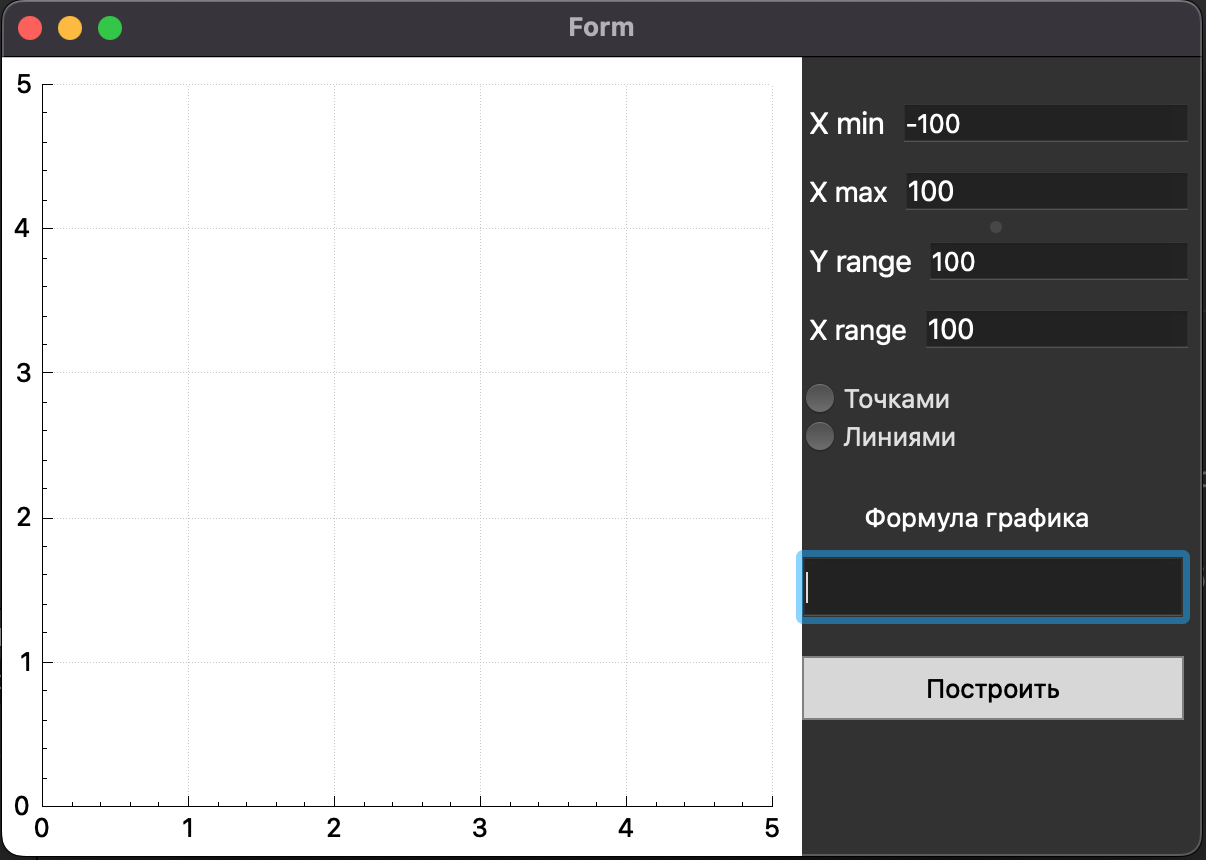
\includegraphics[scale = 0.5]{graph}
	
	\begin{itemize}
		
		\item График можно строить как по чтоскам, так и векторами
		
		\item если перейти краевые значения, то значение устанавливается по умолчанию 
	\end{itemize}
	
\end{document}